\documentclass[journal]{IEEEtran}

\usepackage{blindtext}
\usepackage{cite}
\usepackage{graphicx}
\usepackage{array}
\usepackage{color}
\usepackage{tabularx}
\usepackage{epsfig}
\usepackage{amsmath}
\usepackage{amssymb}
\usepackage{bm}
\usepackage{wasysym}
\usepackage{circuitikz}
\usepackage{float}
\usetikzlibrary{arrows,shapes,calc,positioning}

\newcommand{\myscope}[2]
{\draw[thick,rotate=#2] (#1) circle (12pt)
(#1) ++(-0.35,-0.1) --++ (0.3,0.3) --++ (0,-0.3) --++(0.3,0.3) --++(0,-0.3);}

\begin{document}

\title{CSCE~221 \\ Problem~Set~5}

\author{Jacob~Purcell,~\IEEEmember{Texas~A\&M,~Student}}

\maketitle
\section*{Problem 1}
	Included in ll.cpp.

\section*{Problem 2}
\subsection*{a)}
	Included in ll.cpp.
\subsection*{b)}
	I checked by making my function is a constant member function. So yes it can 
	be done using a constant function. One just has to take care in creating 
	useful getters and setters.

\section*{Problem 3}
	Let us call this pointer to a node an "index." The most apparent way 
	would be to have a cursor pointer iterate up to just before the index. 
	Then, set cursor's next pointer to be indexes next pointer. Index can 
	now be recycled without losing any data. 

	\begin{figure}[h!]
		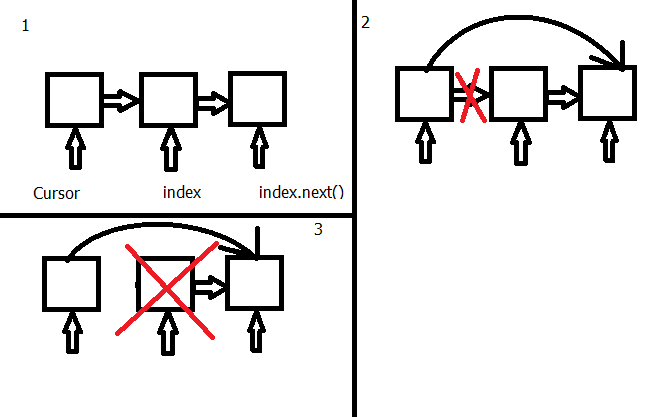
\includegraphics[scale = 0.5]{Untitled.png}
		\caption{Graphical represnetation of the description above.}
	\end{figure}



\end{document}
